% \subsection{Motivation}

\begin{frame}{Scenario}

    \vfill
    \begin{columns}[T,onlytextwidth]
        \begin{column}{0.65\textwidth}
            \begin{figure}
                \includegraphics<1>[width=\textwidth]{figures/scene1.png}%
                \includegraphics<2>[width=\textwidth]{figures/scene2.png}%
                \includegraphics<3>[width=\textwidth]{figures/scene3.png}%
                \includegraphics<4>[width=\textwidth]{figures/scene4.png}%
                \includegraphics<5->[width=\textwidth]{figures/scene5.png}%
            \end{figure}
        \end{column}
        \begin{column}{0.34\textwidth}
            \textbf{Sound}
            \begin{itemize}
                \item<1-> produced by \alert{sources}
                \item<2-> recorded by \alert{microphones}
                \item<3-> corrupted by \alert{noise}
                \only<4>{\item propagates in the \alert{space}}
                \only<5->{\item propagates in the \alert{room}
                          \\$\hookrightarrow$ \alert{reverberation}}
            \end{itemize}
        \end{column}
    \end{columns}

    \vfill
    \visible<6->{
    \textcolor{gray}{Attention: artificial sound vs \textbf{(natural) microphone recordings}}
    }

\end{frame}

\begin{frame}[t]{Echo-aware signal processing for \alert{audio scene analysis}}


    \begin{columns}
        \visible<1->{
        \begin{column}[t]{0.3\textwidth}
            \centering
            \alert{Semantic} information

            \vspace*{0.5em}
            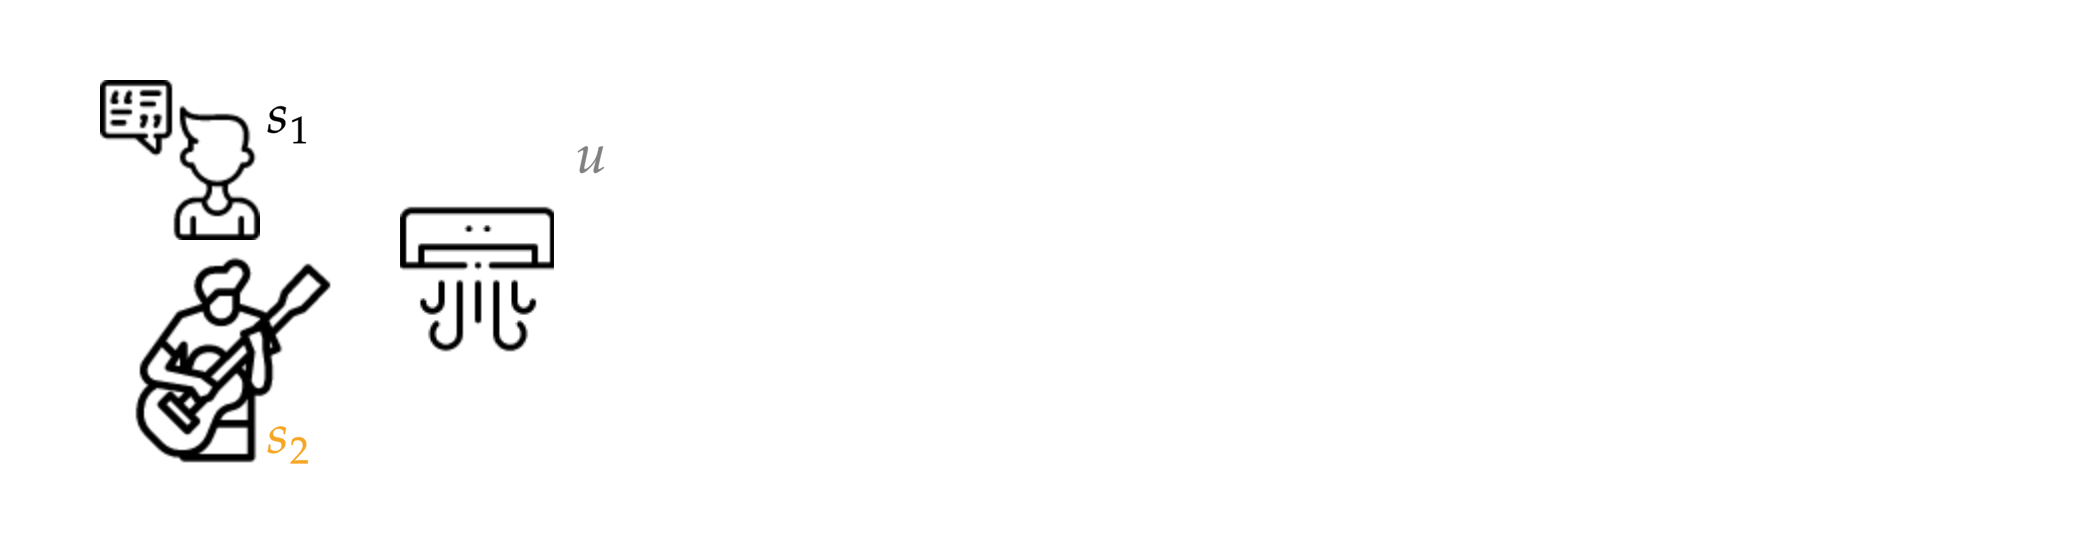
\includegraphics[trim={0 0 170em 0},clip,width=\textwidth]{figures/semantic.png}
        \end{column}}
        \visible<2->{
        \begin{column}[t]{0.3\textwidth}
            \centering
            \alert{Spatial} information

            \vspace*{0.5em}
            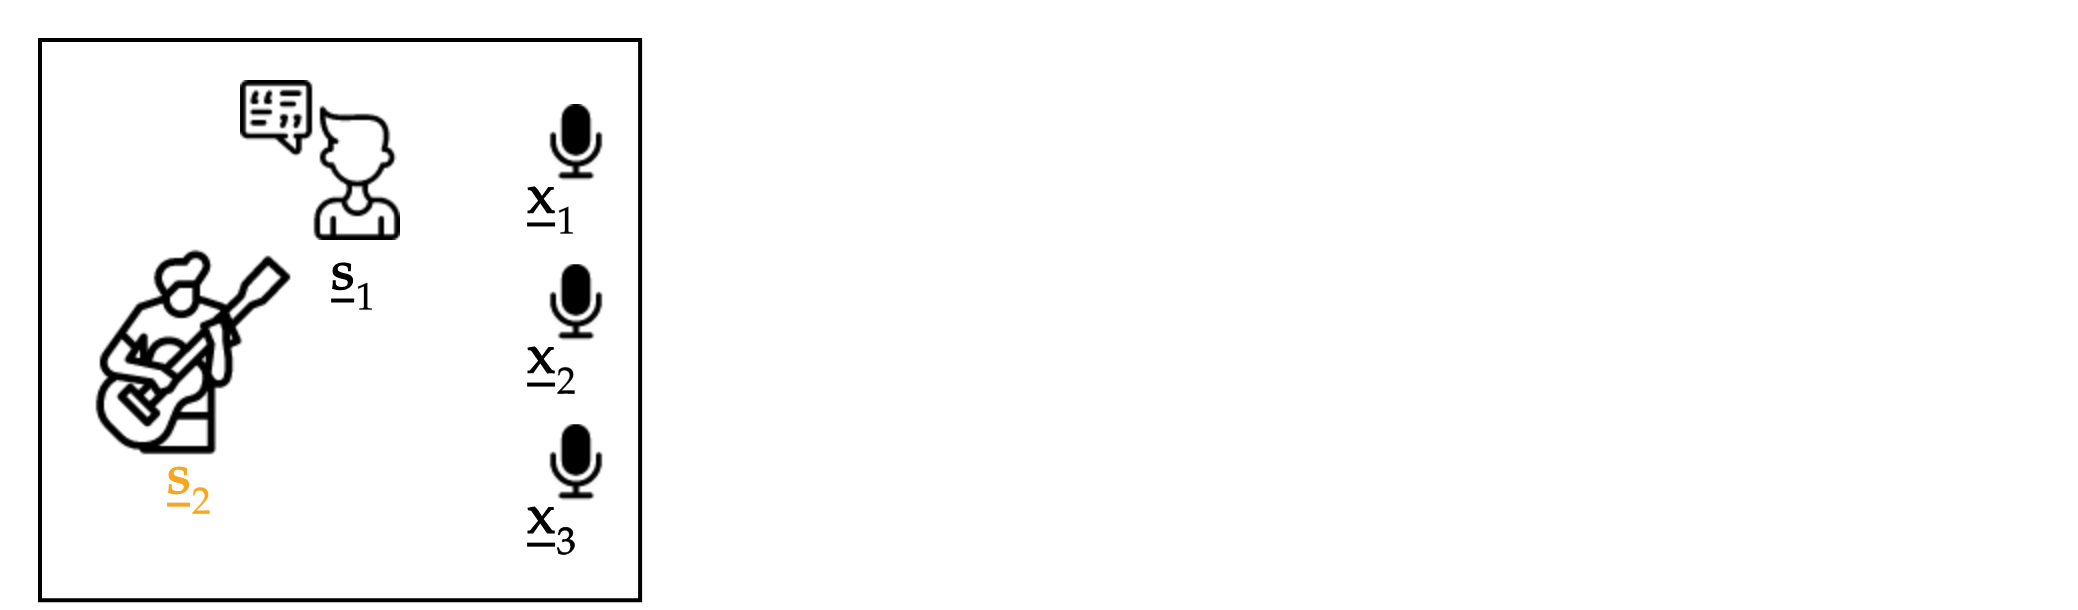
\includegraphics[trim={0 0 170em 0},clip,width=\textwidth]{figures/spatial.png}
        \end{column}}
        \visible<3->{
        \begin{column}[t]{0.3\textwidth}
            \centering
            \alert{Temporal} information

            \vspace*{0.5em}
            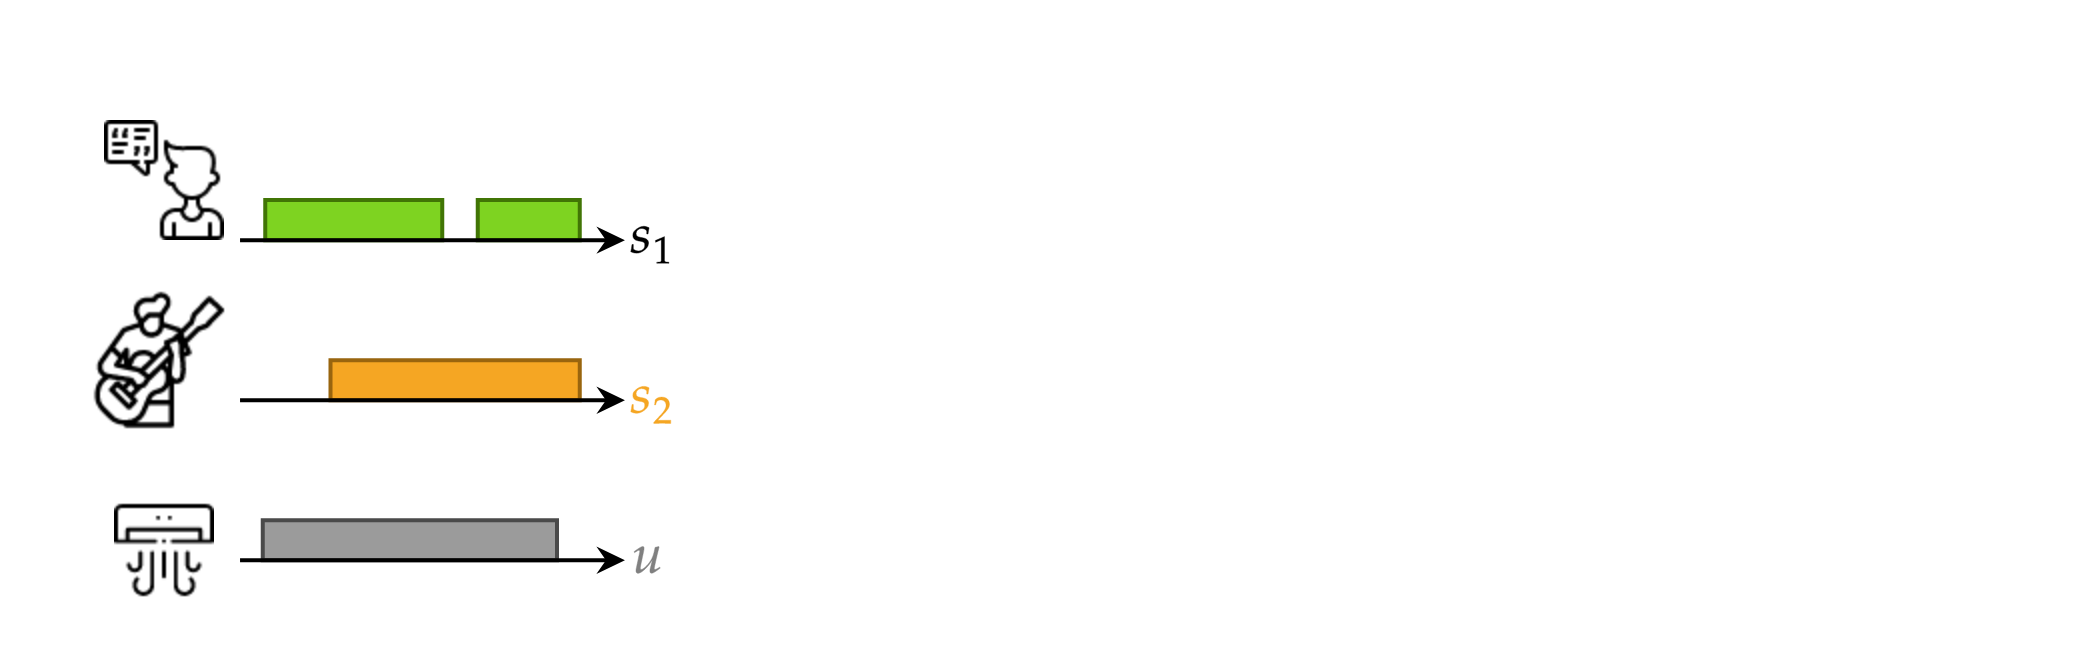
\includegraphics[trim={0 0 170em 0},clip,width=\textwidth]{figures/temporal.png}
        \end{column}}
    \end{columns}

    \begin{columns}
        \visible<1->{
        \begin{column}[t]{0.3\textwidth}
            \centering
            on nature and content
        \end{column}}
        \visible<2->{
        \begin{column}[t]{0.3\textwidth}
            \centering
            on position and geometry
        \end{column}}
        \visible<3->{
        \begin{column}[t]{0.3\textwidth}
            \centering
            on events activity
        \end{column}
        }
    \end{columns}


    \vfill
    \visible<4->{
    \begin{mydefblock}{Audio Scene Analysis}
        Extraction and organization of all the information in the sound
    \end{mydefblock}

    \begin{center}
        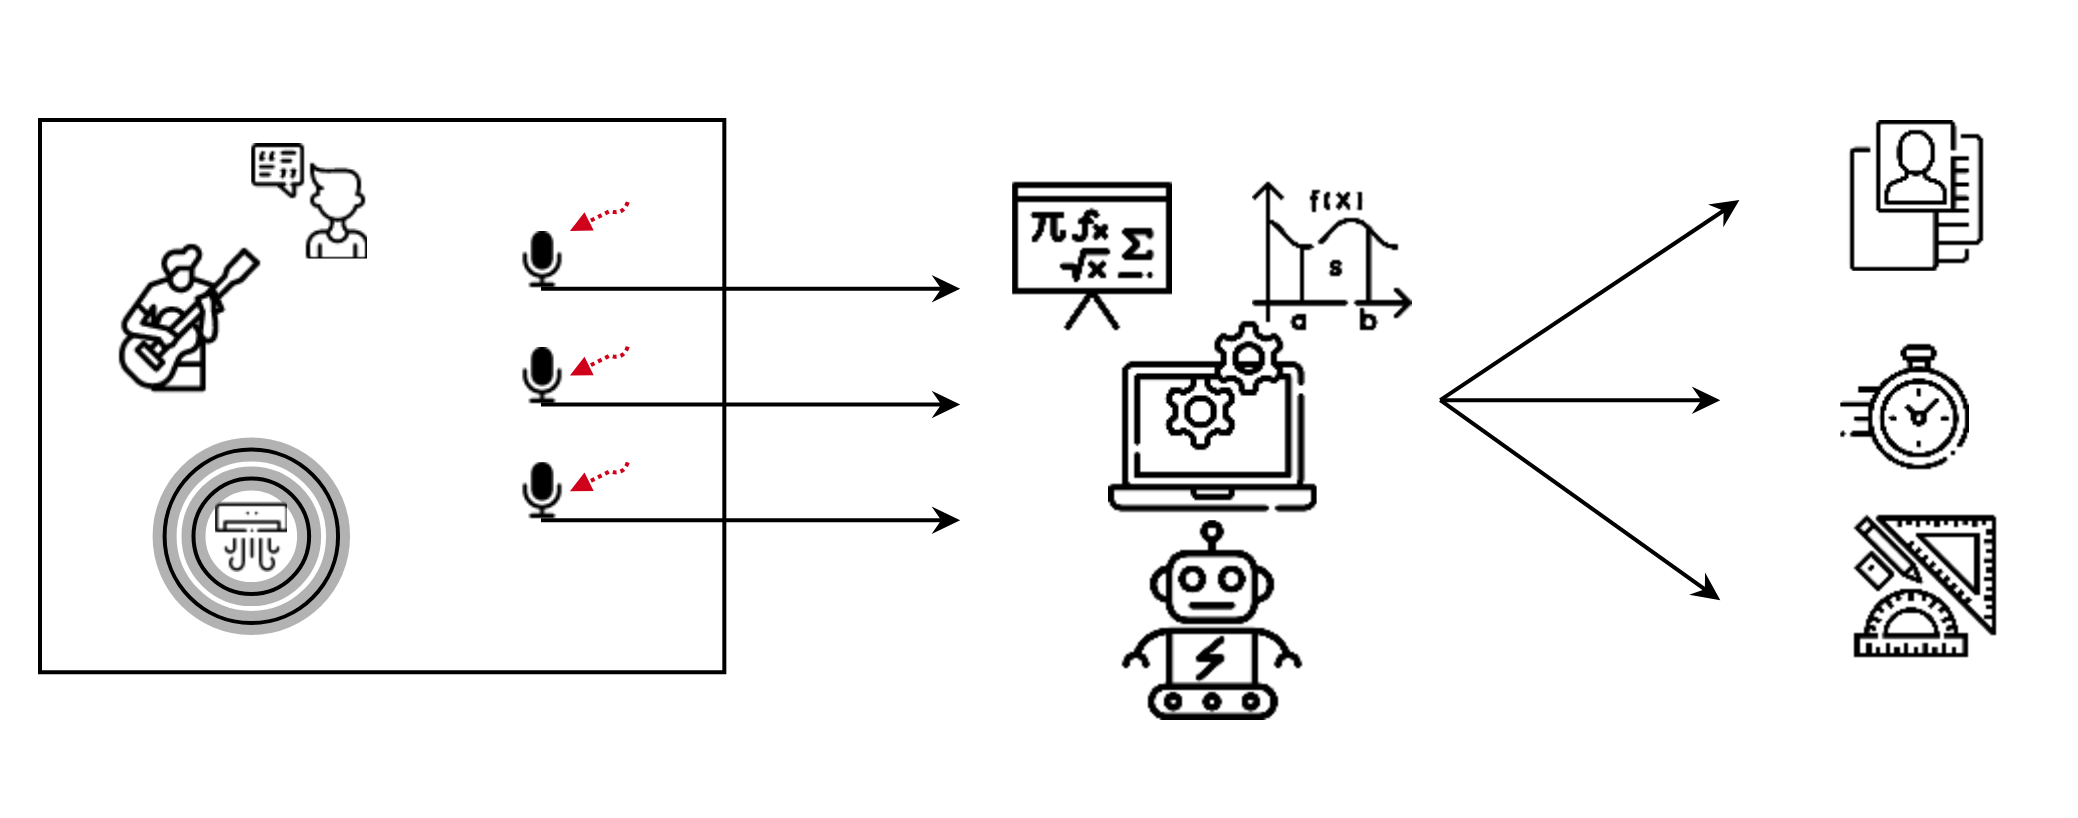
\includegraphics[trim={0 35mm 0 35mm},clip,width=0.8\textwidth]{figures/scene_analysis.png}
    \end{center}
    }

    \only<5->{
    \begin{textblock*}{40mm}(80mm,90mm)
        \textcolor{myred}{\textbf{Can computer do it?}}
    \end{textblock*}
    }

\end{frame}

\begin{frame}[t]{Echo-aware \alert{signal processing for audio scene analysis}}

    \begin{center}
        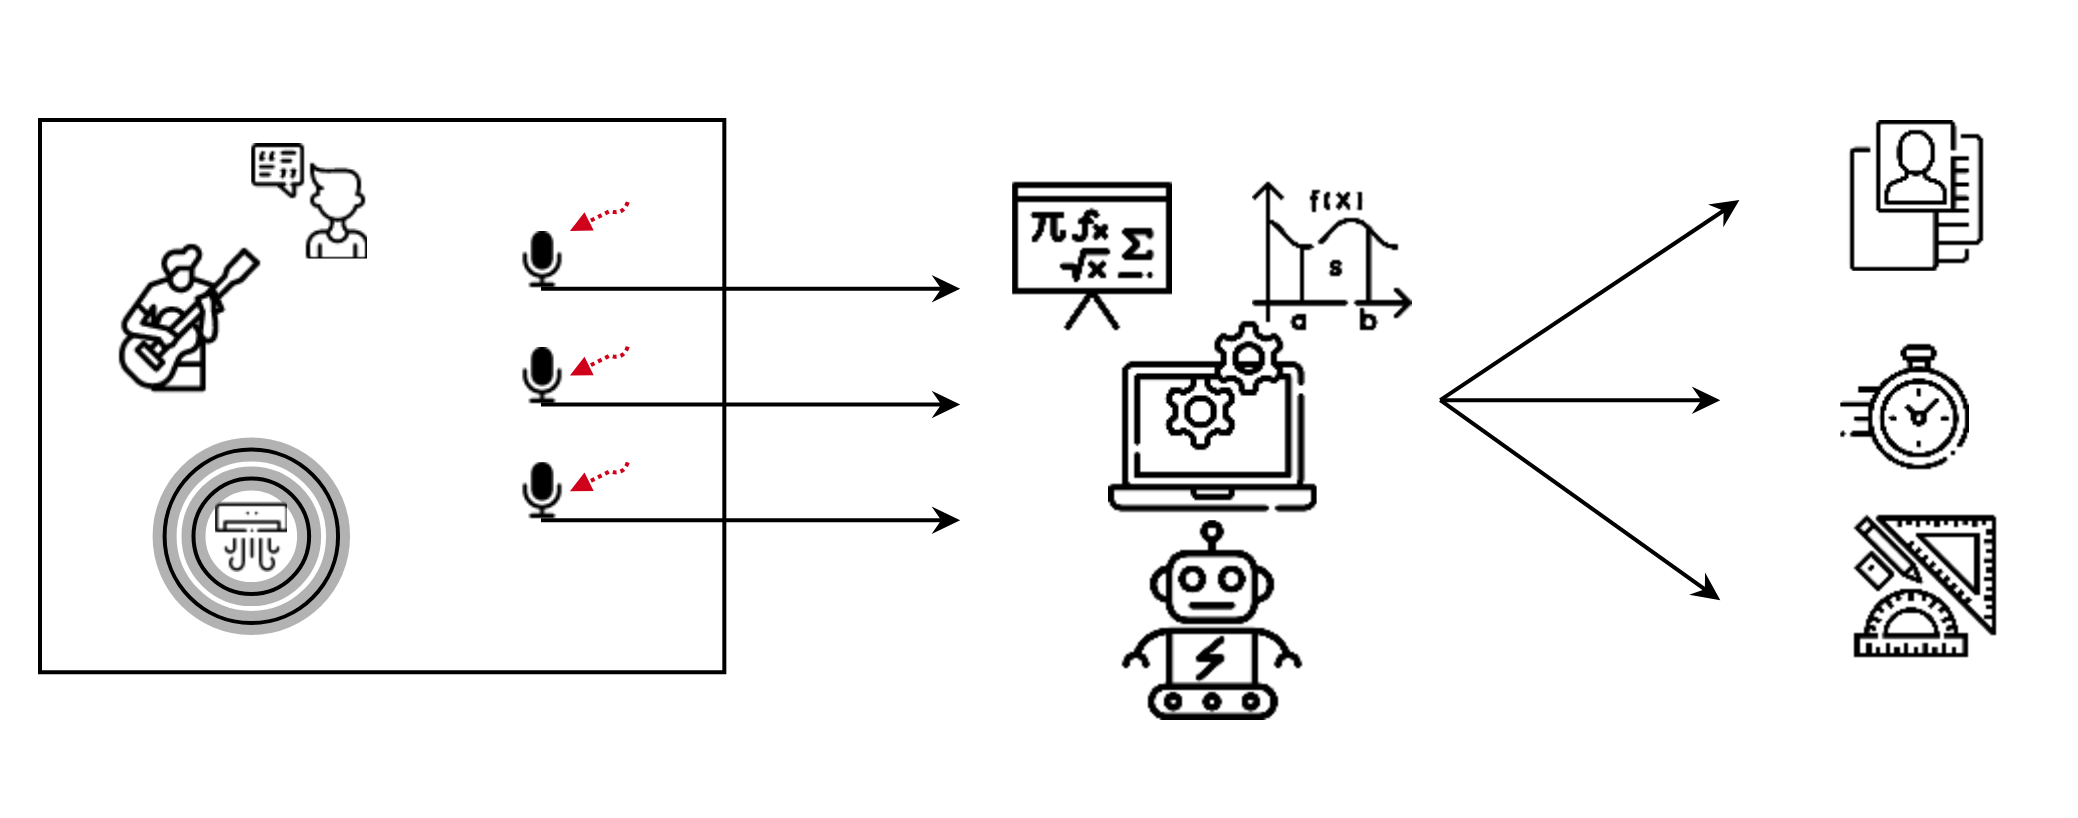
\includegraphics[trim={0 35mm 0 35mm},clip,width=0.8\textwidth]{figures/scene_analysis.png}
    \end{center}

    \pause
    \begin{mydefblock}{Signal Processing}
        Mathematical models, frameworks and tools to tackle and solve such problems
    \end{mydefblock}

    \pause
    {\small Some (inverse) problems}
    \begin{columns}[T,onlytextwidth]
        \begin{column}{0.48\textwidth}
            \small
            \begin{itemize}
                \item Speaker Identification\tikzmark{top1}\tikzmark{bot1}
                \item Sound Source Separation (SSS) \tikzmark{top2}
                \item Speech Enhancement (SE)
                \item Automatic Speech Recognition (ASR)\hspace{0.5em}\tikzmark{right1}\tikzmark{bot2}
                \item Sound Source Localization (SSL) \tikzmark{top3}
                \item Room Geometry Estimation (RooGE)  \tikzmark{bot3}
            \end{itemize}
        \end{column}

        \begin{column}{0.48\textwidth}
            \small
            \begin{itemize}
                \item Voice Activity Detection\tikzmark{top4}
                \item Diarization                \tikzmark{bot4}
                \item RT$_{60}$ estimation       \tikzmark{top5}
                \item Acoustic Channel Estimation\hspace{0.5em}\tikzmark{right2}
                \item Wall Absorption Estimation\tikzmark{bot5}
                \item \textit{and many many other}
            \end{itemize}

        \end{column}
    \end{columns}

    \pause
    \begin{tikzpicture}[overlay, remember picture]
        \node[anchor=base] (a) at (pic cs:top1) {\vphantom{h}}; % push the mark to the top of the line (ie including ascenders)
        \node[anchor=base] (b) at (pic cs:bot1) {\vphantom{g}}; % push the mark to the bottom of the line (ie including descenders)
        \draw [decoration={brace,amplitude=0.5em},decorate,thick,gray]
         (a.north -| {pic cs:right1}) -- node[right,inner sep=1em] {\small Who?} (b.south -| {pic cs:right1});
    \end{tikzpicture}
    \begin{tikzpicture}[overlay, remember picture]
        \node[anchor=base] (a) at (pic cs:top2) {\vphantom{h}}; % push the mark to the top of the line (ie including ascenders)
        \node[anchor=base] (b) at (pic cs:bot2) {\vphantom{g}}; % push the mark to the bottom of the line (ie including descenders)
        \draw [decoration={brace,amplitude=0.5em},decorate,thick,gray]
         (a.north -| {pic cs:right1}) -- node[right,inner sep=1em] {\small What?} (b.south -| {pic cs:right1});
    \end{tikzpicture}
    \begin{tikzpicture}[overlay, remember picture]
        \node[anchor=base] (a) at (pic cs:top3) {\vphantom{h}}; % push the mark to the top of the line (ie including ascenders)
        \node[anchor=base] (b) at (pic cs:bot3) {\vphantom{g}}; % push the mark to the bottom of the line (ie including descenders)
        \draw [decoration={brace,amplitude=0.5em},decorate,thick,gray]
         (a.north -| {pic cs:right1}) -- node[right,inner sep=1em] {\small Where?} (b.south -| {pic cs:right1});
    \end{tikzpicture}
    \begin{tikzpicture}[overlay, remember picture]
        \node[anchor=base] (a) at (pic cs:top4) {\vphantom{h}}; % push the mark to the top of the line (ie including ascenders)
        \node[anchor=base] (b) at (pic cs:bot4) {\vphantom{g}}; % push the mark to the bottom of the line (ie including descenders)
        \draw [decoration={brace,amplitude=0.5em},decorate,thick,gray]
         (a.north -| {pic cs:right2}) -- node[right,inner sep=1em] {\small When?} (b.south -| {pic cs:right2});
    \end{tikzpicture}
    \begin{tikzpicture}[overlay, remember picture]
        \node[anchor=base] (a) at (pic cs:top5) {\vphantom{h}}; % push the mark to the top of the line (ie including ascenders)
        \node[anchor=base] (b) at (pic cs:bot5) {\vphantom{g}}; % push the mark to the bottom of the line (ie including descenders)
        \draw [decoration={brace,amplitude=0.5em},decorate,thick,gray]
         (a.north -| {pic cs:right2}) -- node[right,inner sep=1em] {\small How?} (b.south -| {pic cs:right2});
    \end{tikzpicture}

    \pause
    \vspace{-2mm}
    \begin{center}
        HOW  $\overset{\text{helps}}{\longrightarrow}$ WHERE
             $\overset{\text{helps}}{\longrightarrow}$ WHEN
             $\overset{\text{helps}}{\longrightarrow}$ WHAT
             $\overset{\text{helps}}{\longrightarrow}$ HOW
             $\overset{\text{helps}}{\longrightarrow}$ ...
    \end{center}

\end{frame}


% \begin{frame}{Echo-aware \alert{signal processing} for audio scene analysis}

%     \vfill
%     \begin{block}{Signal Model}
%         \begin{columns}
%             \begin{column}{0.45\textwidth}
%                 \centering
%                 \includegraphics[width=0.5\textwidth]{example-image-a}
%             \end{column}
%             \begin{column}{0.58\textwidth}
%                 \begin{itemize}
%                     \item produced by sources
%                     \item propagates in the room
%                     \item corrupted by noise
%                     \item recorded by microphone
%                 \end{itemize}
%             \end{column}
%         \end{columns}
%     \end{block}

% \end{frame}

\begin{frame}[t]{\alert{Echo-aware signal processing for audio scene analysis}}

    \visible<1->{
    \begin{mydefblock}{Acoustic Echoes}

        \vspace{-3mm}
        \begin{columns}[onlytextwidth]
            \begin{column}{0.60\textwidth}
                \begin{itemize}
                    \item Elements of the sound propagation
                    \item Standing out for time and strength
                    \item Repetition of a sound but later
                    \item Both outdoor and indoor
                \end{itemize}
            \end{column}
            \begin{column}{0.38\textwidth}
                \centering
                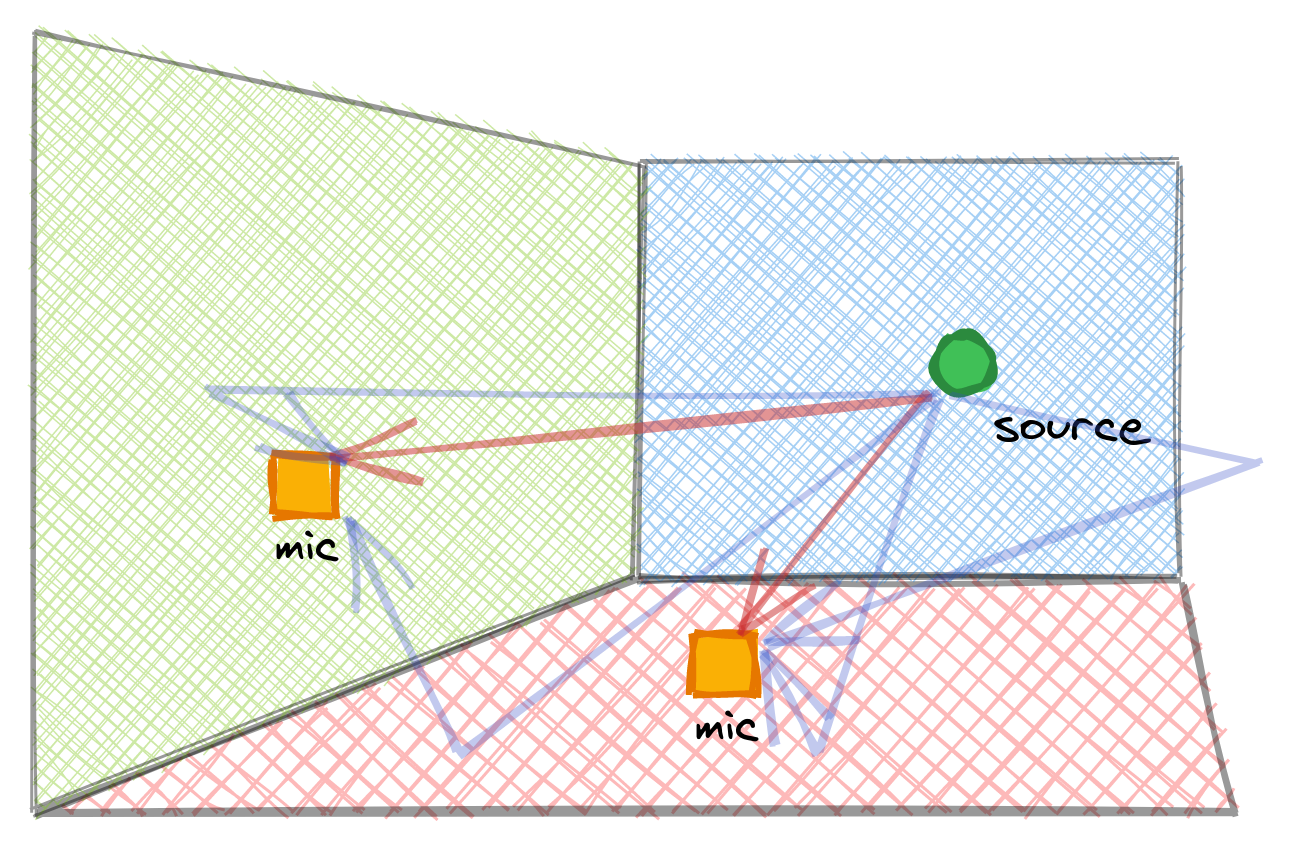
\includegraphics[width=.8\textwidth]{figures/echoes}
            \end{column}

        \end{columns}
    \end{mydefblock}
    }

    \vfill
    \begin{columns}[T,onlytextwidth]
        \begin{column}{0.60\textwidth}
            \begin{block}{Audio signal processing methods}
                    \begin{itemize}
                        \item<3-> \alert{ignore} it
                        \item<4-> assume it \alert{free-field}
                        \item<5-> model it \alert{entirely}
                        \item<6-> model as \alert{few reflection}\tikzmark{top6}
                        \item<7-> model it as \alert{early and late} parts\hspace{1em}\tikzmark{right6}\tikzmark{bot6}
                    \end{itemize}
            \end{block}
        \end{column}
        \begin{column}{0.38\textwidth}
            \only<3>{\adjincludegraphics[Clip={.00\width} {0\height} {.80\width} {0\height},width=\textwidth]{figures/prop_it.png}}%
            \only<4>{\adjincludegraphics[Clip={.20\width} {0\height} {.60\width} {0\height},width=\textwidth]{figures/prop_it.png}}%
            \only<5>{\adjincludegraphics[Clip={.40\width} {0\height} {.40\width} {0\height},width=\textwidth]{figures/prop_it.png}}%
            \only<6>{\adjincludegraphics[Clip={.60\width} {0\height} {.20\width} {0\height},width=\textwidth]{figures/prop_it.png}}%
            \only<7->{\adjincludegraphics[Clip={.80\width} {0\height} {.00\width} {0\height},width=\textwidth]{figures/prop_it.png}}%
        \end{column}
        \end{columns}

    \only<8->{
        \begin{tikzpicture}[overlay, remember picture]
            \node[anchor=base] (a) at (pic cs:top6) {\vphantom{h}}; % push the mark to the top of the line (ie including ascenders)
            \node[anchor=base] (b) at (pic cs:bot6) {\vphantom{g}}; % push the mark to the bottom of the line (ie including descenders)
            \draw [decoration={brace,amplitude=0.5em},decorate,thick,gray]
            (a.north -| {pic cs:right6}) -- node[right,inner sep=1em] {
                \textcolor{myred}{\textbf{Echo-aware methods}}} (b.south -| {pic cs:right6});
        \end{tikzpicture}
    }

    \visible<9->{
        \begin{block}{Modelling the sound field}
            \begin{itemize}
                \item as free field $\implies$ reverberation is noise
                \item entirely $\implies$ it is very challenging
            \end{itemize}
        \end{block}
    }

    % \vfill
    % \begin{block}{Echo-aware processing}
    % \end{block}

    % \begin{columns}[T,onlytextwidth]
    %     \begin{column}{0.3\textwidth}
    %         \alert{Free-field} processing
    %         \\{\small(only direct path)}
    %     \end{column}\hfill
    %     \begin{column}{0.3\textwidth}
    %         \alert{Echo} processing
    %         \\{\small(only specular reflection)}
    %     \end{column}\hfill
    %     \begin{column}{0.3\textwidth}
    %         \alert{Reverberant} processing
    %         \\{\small(entire sound field)}
    %     \end{column}
    % \end{columns}%

    % \vfill
    % \begin{columns}[T,onlytextwidth]
    %     \begin{column}{0.3\textwidth}
    %         \small
    %         \begin{itemize}
    %             \item[\cmark] \textcolor{mygreen}{``simple'' processing} %closed-from formulas %fully deterministic
    %             \item[\cmark] \textcolor{mygreen}{``short'' processing} % STFT, no latency
    %             \item[\xmark] \textcolor{myred}{Reflection are interferences}
    %             \item[\xmark] \textcolor{myred}{Neglect most of the sound energy}
    %             \item[\xmark] \textcolor{myred}{incoherence $\implies$ distortion}
    %         \end{itemize}
    %     \end{column}\hfill
    %     \begin{column}{0.3\textwidth}
    %         \small
    %         \begin{itemize}
    %             \item short processing %  echoes $\rightleftarrows$ positions
    %             \item simple processing
    %             \item reflection are integrated,
    %             \\late reverberation can considered
    %             \item reflection are difficult to estimate
    %             \item reflection need to be correctly estimated
    %         \end{itemize}
    %     \end{column}\hfill
    %     \begin{column}{0.3\textwidth}
    %         \small
    %         \begin{itemize}
    %             % fully deterministic and stochastic processing
    %             \item difficult processing %estimation is extremely difficult, more parameters to estimate
    %             \item long precessing
    %             \item Reflection perfectly integrated
    %         \end{itemize}
    %     \end{column}
    % \end{columns}

    %     \\Anechoic processing
    %     \begin{itemize}
    %         \item short processing
    %         \item[\cmark] sound field tends to be diffuse
    %         \item[\xmark] sound reflection as interferences
    %         \\neglect most of the sound energy
    %         \\ignore the correlation between the direct sound and its reflection and consequently may result in a distorted output
    %         \item[\xmark] coherent processing becomes impossible
    %     \end{itemize}
    %     Echo-processing
    %     \begin{itemize}
    %         \item Middle processing
    %         perceive coming from all directions~\cite{daldegan1988}
    %     \end{itemize}
    %     Reverberant processing
    %     \begin{itemize}
    %         \item Long processing
    %         \item[\cmark] narrowband approximation is valid
    %         \item[\cmark] sound field is described by full RIRs
    %         \item[\cmark] all reflection can be \alert{coherently} processed
    %         \item[\xmark] long frames impose lantency
    %     \end{itemize}
    % \end{block}

\end{frame}

\begin{frame}{Goals and contributions}

    \begin{columns}[onlytextwidth]
        \begin{column}[T]{0.3\linewidth}
            \centering
            \textbf{Audio Scene Analysis}
            \\\downarrow
            \\context and problems
        \end{column}\hfill\pause
        \begin{column}[T]{0.3\linewidth}
            \centering
            \textbf{Signal Processing}
            \\\downarrow
            \\models and frameworks
        \end{column}\hfill\pause
        \begin{column}[T]{0.3\linewidth}
            \centering
            \textbf{Acoustic Echoes}
            \\\downarrow
            \\better processing
        \end{column}\hfill
    \end{columns}
    \pause

    \vfill
    \begin{mydefblock}{Goals}
        \begin{enumerate}
            \item How to \textbf{estimate} acoustic echoes?
            \item How to \textbf{extend methods} for echo-aware audio scene analysis
        \end{enumerate}
    \end{mydefblock}
    \pause

    \vfill
    \begin{columns}[T,onlytextwidth]
        \begin{column}{0.48\textwidth}
            \centering
            \textbf{1. Estimation}
        \end{column}
        \begin{column}{0.48\textwidth}
            \centering
            \textbf{2. Application}
        \end{column}
    \end{columns}

    \pause
    \begin{columns}[T]
        \begin{column}{0.48\textwidth}
            \begin{itemize}
                \item Knowledge-based echo estimation
                \\$\hookrightarrow$ \blaster
                \item Learning-based echo estimation
                \\$\hookrightarrow$ \lantern
            \end{itemize}
        \end{column}
        \pause
        \begin{column}{0.48\textwidth}
            \begin{itemize}
                \item Echo-aware Source Separation
                \\$\hookrightarrow$ \separake
                \item Echo-aware Source Localization
                \\$\hookrightarrow$ \mirage
                \item Echo-aware Speech Enhancement
                \item Echo-aware Room Geometry Estimation
            \end{itemize}
        \end{column}
    \end{columns}
    \pause
    \begin{center}
        \textbf{3. Data:}
        \\Echo-aware database $\rightarrow$ \dechorate
    \end{center}
\end{frame}

% % change color of Beamer subsection
% % https://tex.stackexchange.com/questions/356237/changing-text-color-in-subsection-in-tableofcontents-in-beamer
% \begin{frame}[standout]{1D Outline}
%     \begin{columns}
%         \begin{column}{0.35\textwidth}
%             Echo-aware signal processing
%             \\for audio scene analysis
%         \end{column}
%         \begin{column}{0.05\textwidth}
%         \end{column}
%         \begin{column}{0.6\textwidth}
%             {
%                 \setbeamercolor{part in toc}{fg=gray}
%                 \setbeamercolor{section in toc}{fg=gray}
%                 \setbeamercolor{subsection in toc}{fg=white}
%                 \tableofcontents
%             }
%         \end{column}
%     \end{columns}
% \end{frame}